\chapter{Habitat of ice reservoirs}

\cleanchapterquote{Ice stupas offer a solution to the shortage of water all our mountain regions are
facing.}{Pema Gyamtsho }{(Director General, International Center for Integrated Mountain Development)}

AIRs cannot be built anywhere. They require favourable weather conditions, sufficient water supply, and specific
topography to amass a seasonal stock of ice. However, these three requirements can vary drastically both
temporally and spatially. Therefore, datasets of high resolution are necessary to judge any location's AIR
suitability. 

In this chapter, we base our analysis on the ice stupas built in Swiss and the Indian regions where such
datasets are available. We examine their observed volume variations in different spatial and temporal scales .
Later, we discuss some useful metrics to qualitatively assess the suitability of new construction locations in a
regional and local scale.

\section{Observed ice volume variability}

\subsection{Interregional scale}

% \begin{figure}[htb]
% \centering
% 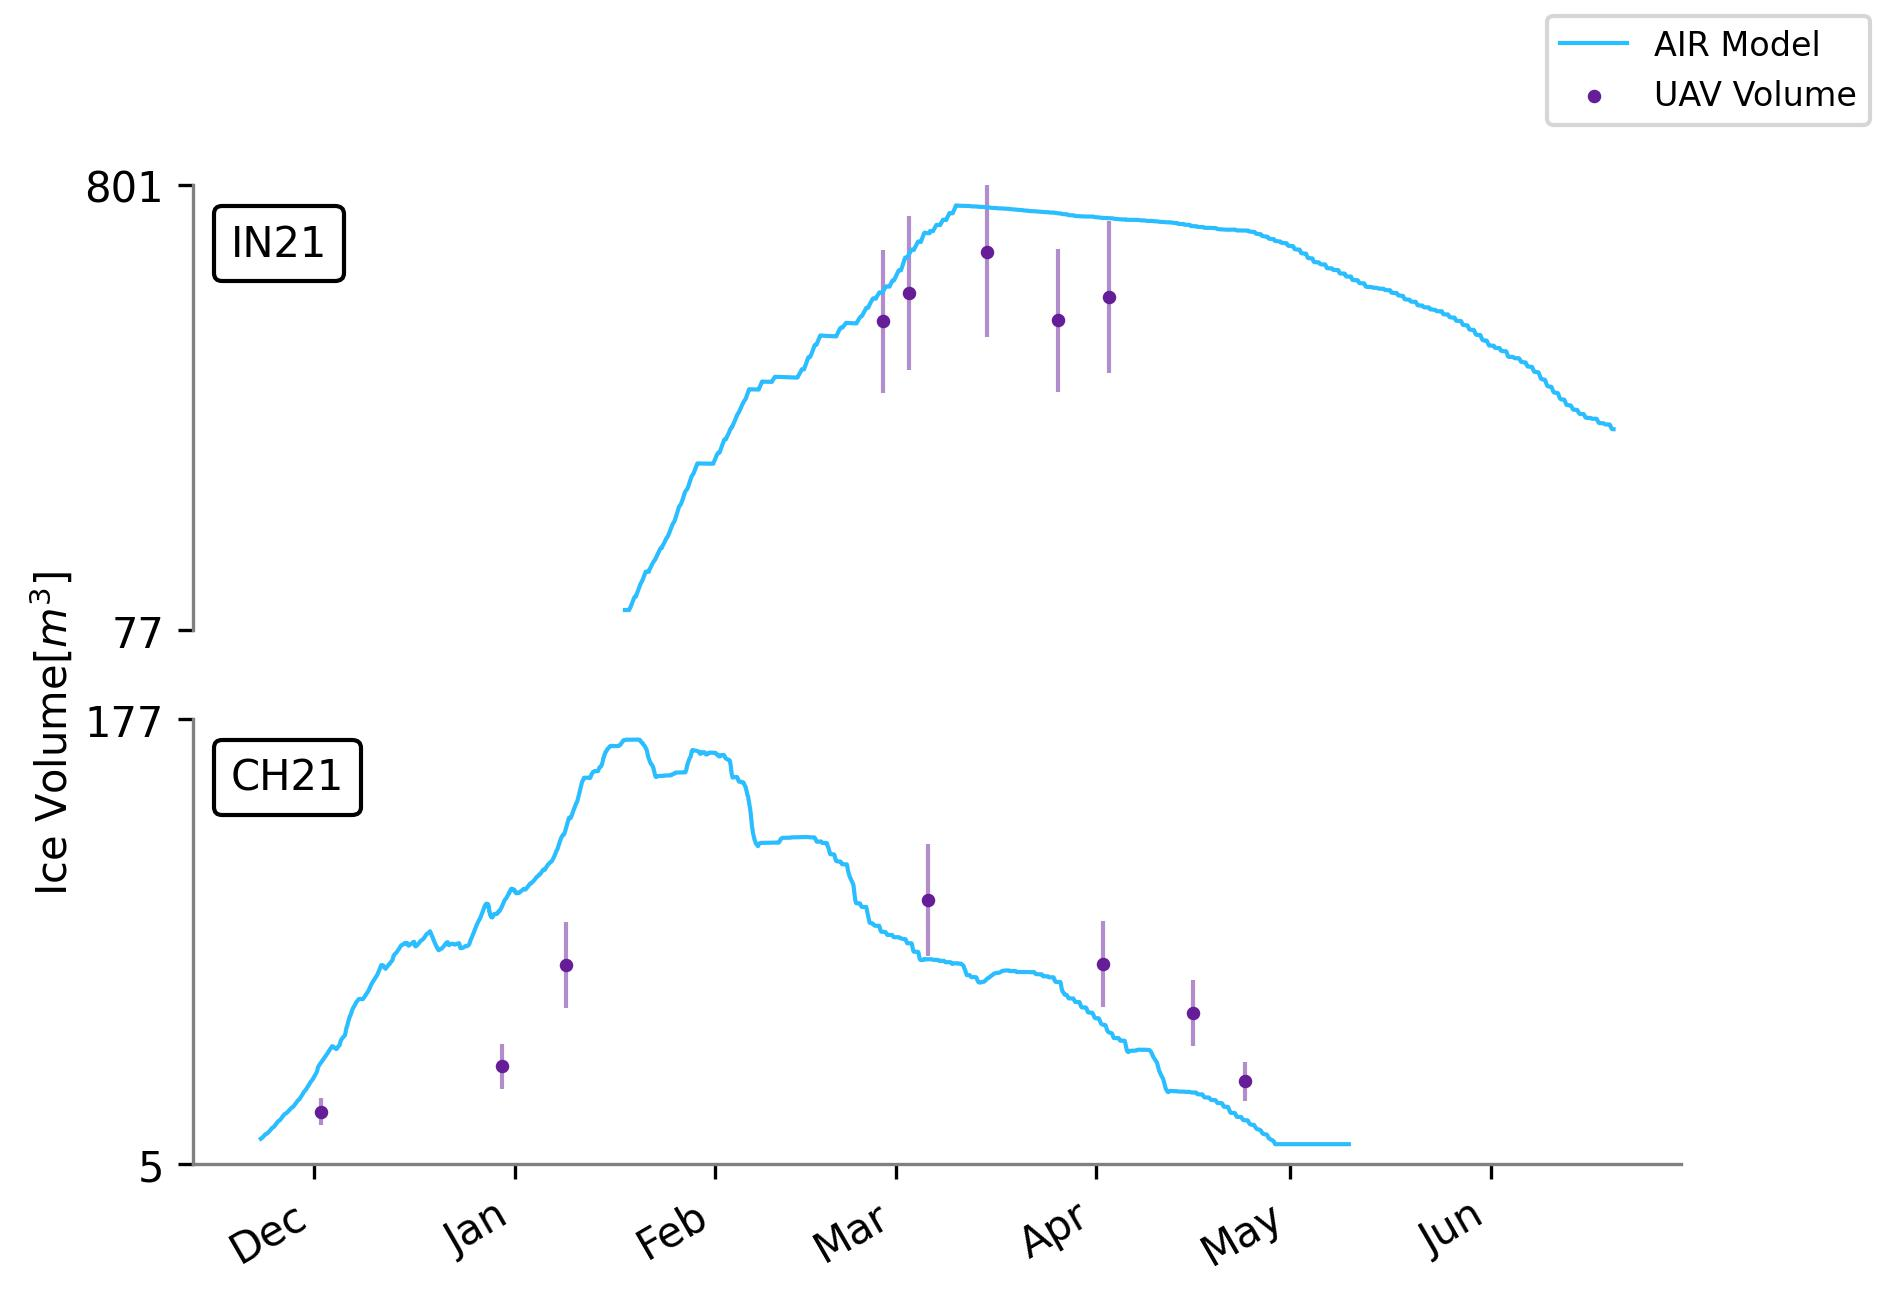
\includegraphics[width=\textwidth]{figs/IN21vsCH21.jpg}
% \caption{AIRs show significant variation in volume evolution depending on the choice of construction location.}
% \label{fig:2AIRs}
% \end{figure}

Ice stupa volumes and survival duration show drastic variation between the Swiss Alps and Indian Himalayas.
Comparison of ice stupa volume evolution show that Indian ones grew four times larger than Swiss ones (  Fig.
\ref{fig:2AIRs}). The corresponding freezing rate of the Indian ice stupa was more than ten times higher than the
Swiss. Sublimation was identified as the driving process of this difference (  paper II). Therefore, the
colder, drier and less cloudy weather characteristics of the Ladakh region made it more suitable to build AIRs
compared to the Guttannen region. 

\subsection{Intraregional scale}

\begin{figure}[htb]
	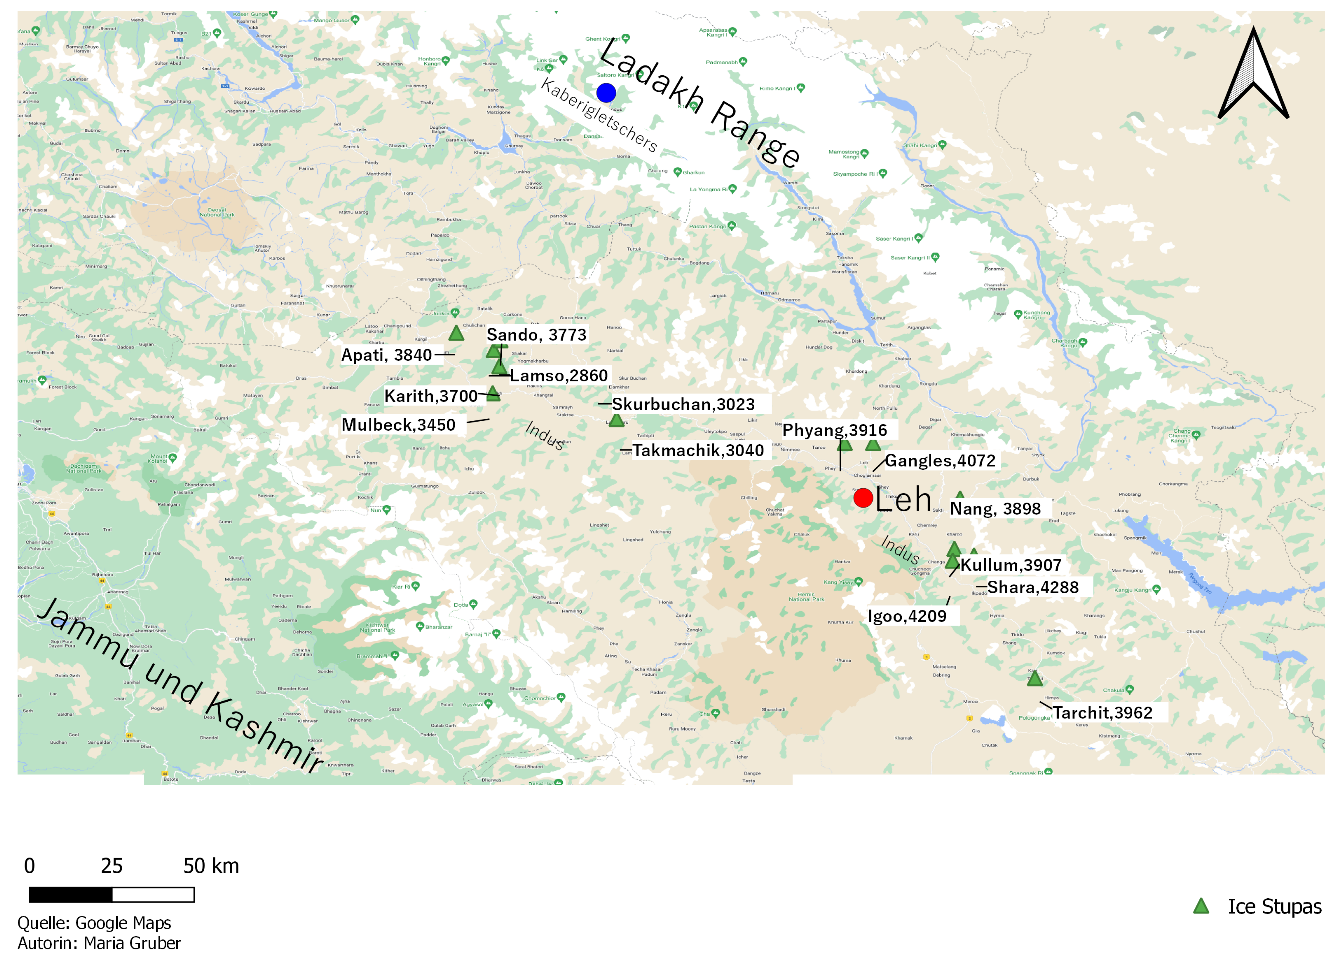
\includegraphics[width=\textwidth]{figs/ISC_villages}
  \caption{Some villages of Ladakh, India where AIRs are built.}
	\label{fig:villages}
\end{figure}

Over the past decade more than 14 villages in Ladakh have built ice stupas (Fig. \ref{fig:villages}). Their
volume variation reveals a correlation with the altitude of the construction location (Fig. \ref{fig:altvsvol}).
This correlation indicates that elevation gain of 100 $m$ causes a corresponding ice volume gain of 1 million
litres. However, some locations with lower altitude exhibit higher volumes compared to those with a higher
altitude. This is due to topographic effects of shadow valleys that reduce the sunshine hours of the location
(\cite{Maria}).

\begin{figure}[htb]
\centering
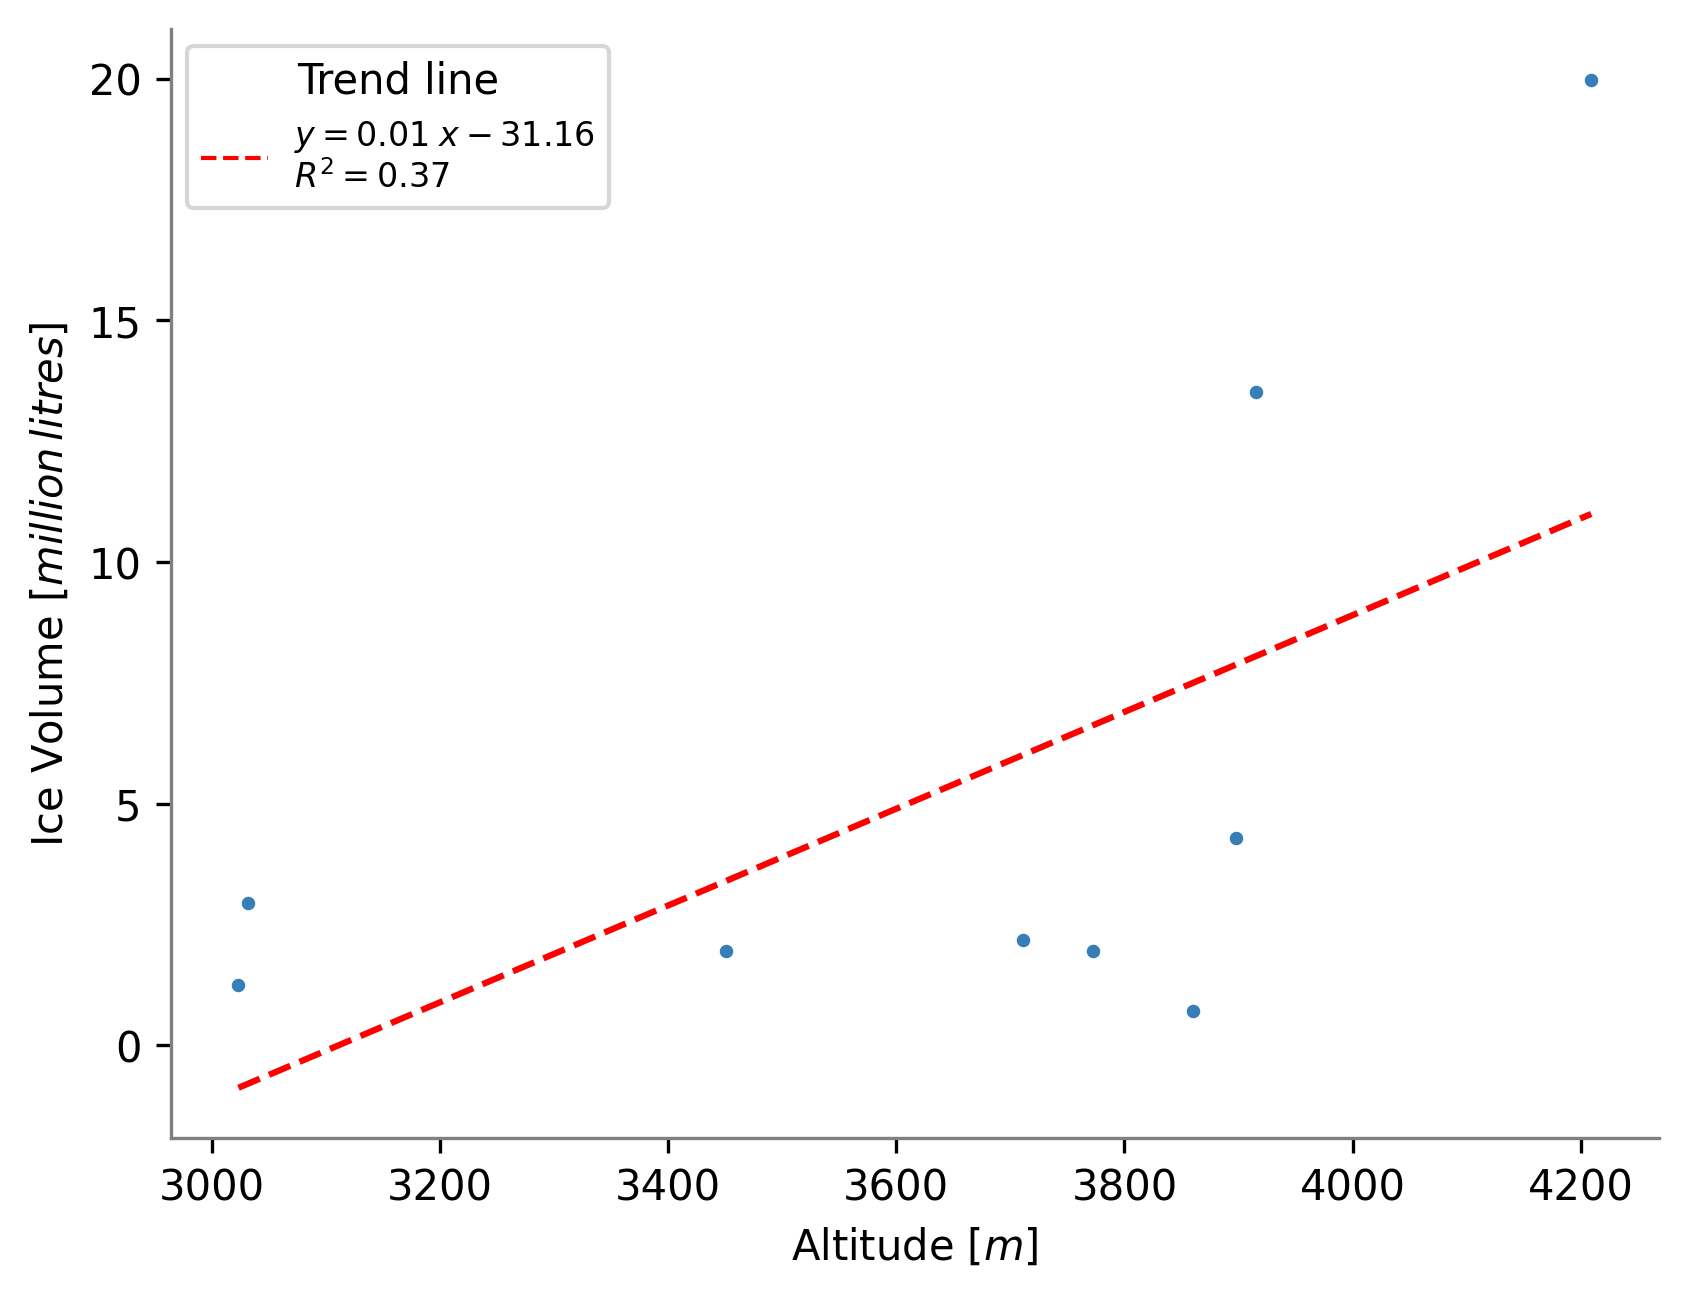
\includegraphics[width=\textwidth]{figs/altitudevsvolume.png}
\caption{Relationship of measured ice volume with altitude of AIRs built during winter of 2019-20 across
different villages in Ladakh. Adapted from Maria  }
\label{fig:altvsvol}
\end{figure}

Some ice stupas built in villages above 4200 m a.s.l. (Shara and Igoo) have also been observed to last beyond a
summer melt season (Fig. \ref{fig:PIR}). However, Swiss locations having such favourable weather conditions
remain to be discovered. A possible way to study this question is to decrease the air temperature uniformly
(temperature change $\Delta T$). This will imply a stronger negative sensible heat flux in summer, thus
accelerating icestupa growth and slowing down its decay. Such simulations were produced in paper III for an ice
stupa grown in the Diavolezza site at an altitude of 2080 m a.s.l. . We found a break-even point for $\Delta T = -2 \degree
C$ (Fig. \ref{fig:PIR_evolution}). For larger negative values of $\Delta T$ the icestupa does not disappear in
summer and keeps growing from year to year. For $\Delta T = -3 \degree C$, the maximum volume in the fifth year
is about 4 times that in the first year (  Fig. \ref{fig:PIR}). Therefore, ice stupas can compound in size if
built in Swiss locations with an elevation above 2388 $m$ (based on a standard atmospheric lapse rate of 0.0065
$\degree\,C\,m^{-1}$) .

\begin{figure}[htb]
  \centering
	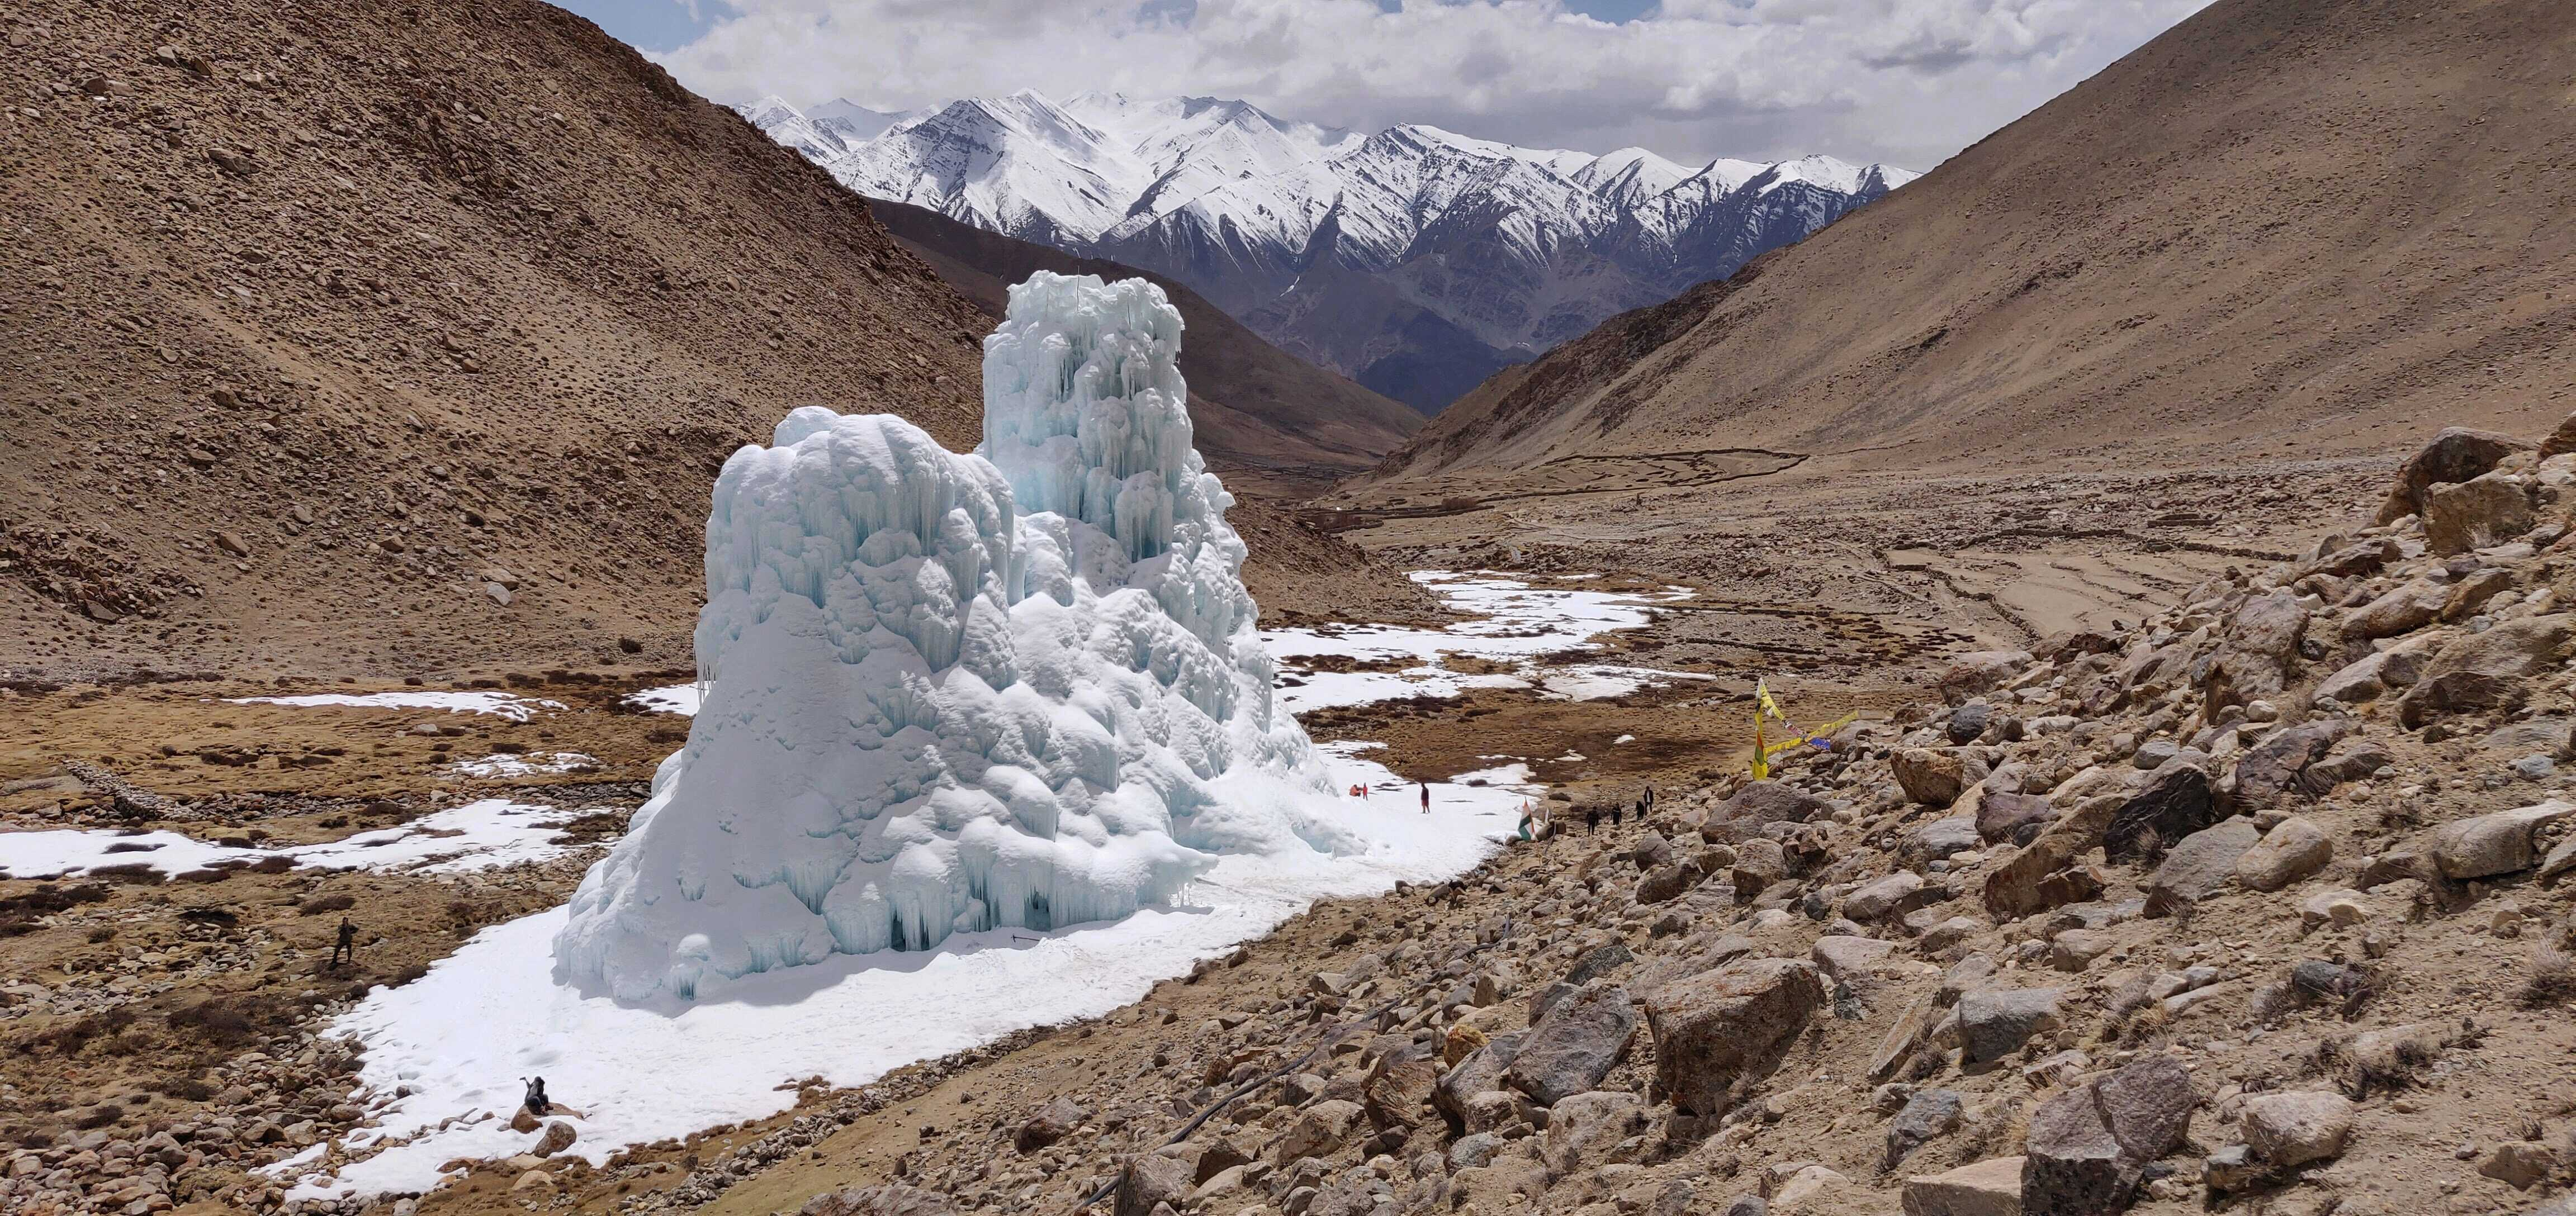
\includegraphics[width=\textwidth]{figs/PIR_example.jpg}

  \caption{Icestupa at Shara, Ladakh, built by local farmers in the winter of 2019-20, survived a full summer melt season and released
  around 8 million litres of water.} 

\label{fig:PIR} 
\end{figure}

\begin{figure}[htb]
  \centering
	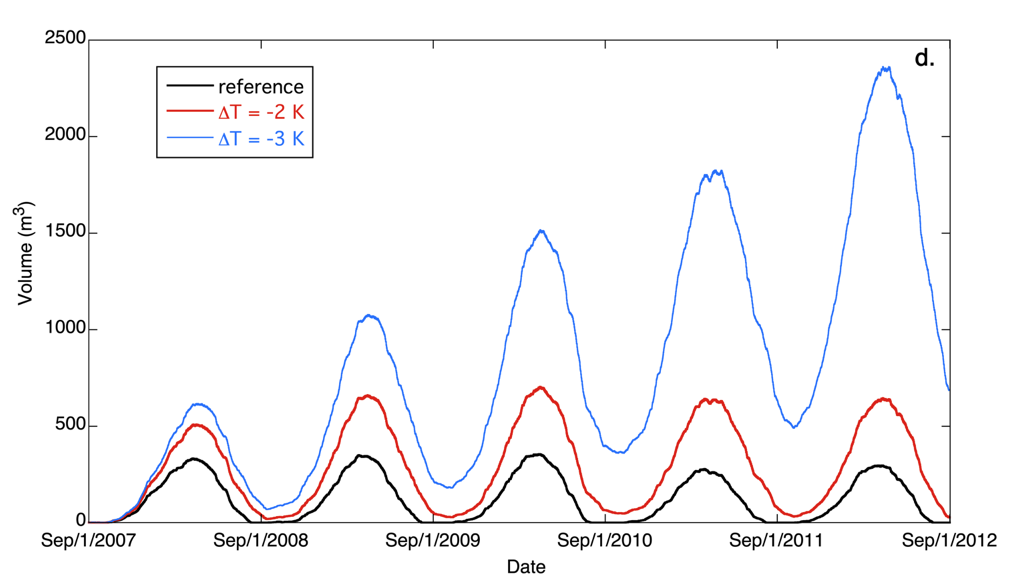
\includegraphics[width=\textwidth]{figs/PIR_evolution.png}
  \caption{The effect of a negative temperature perturbation. For $\Delta T = -3 \degree C$ the icestupa does
  not disappear anymore but is growing from year to year.}
\label{fig:PIR_evolution}
\end{figure}

\subsection{Interannual scale}
\label{sec:interannual}

\begin{figure}[htb]
\centering
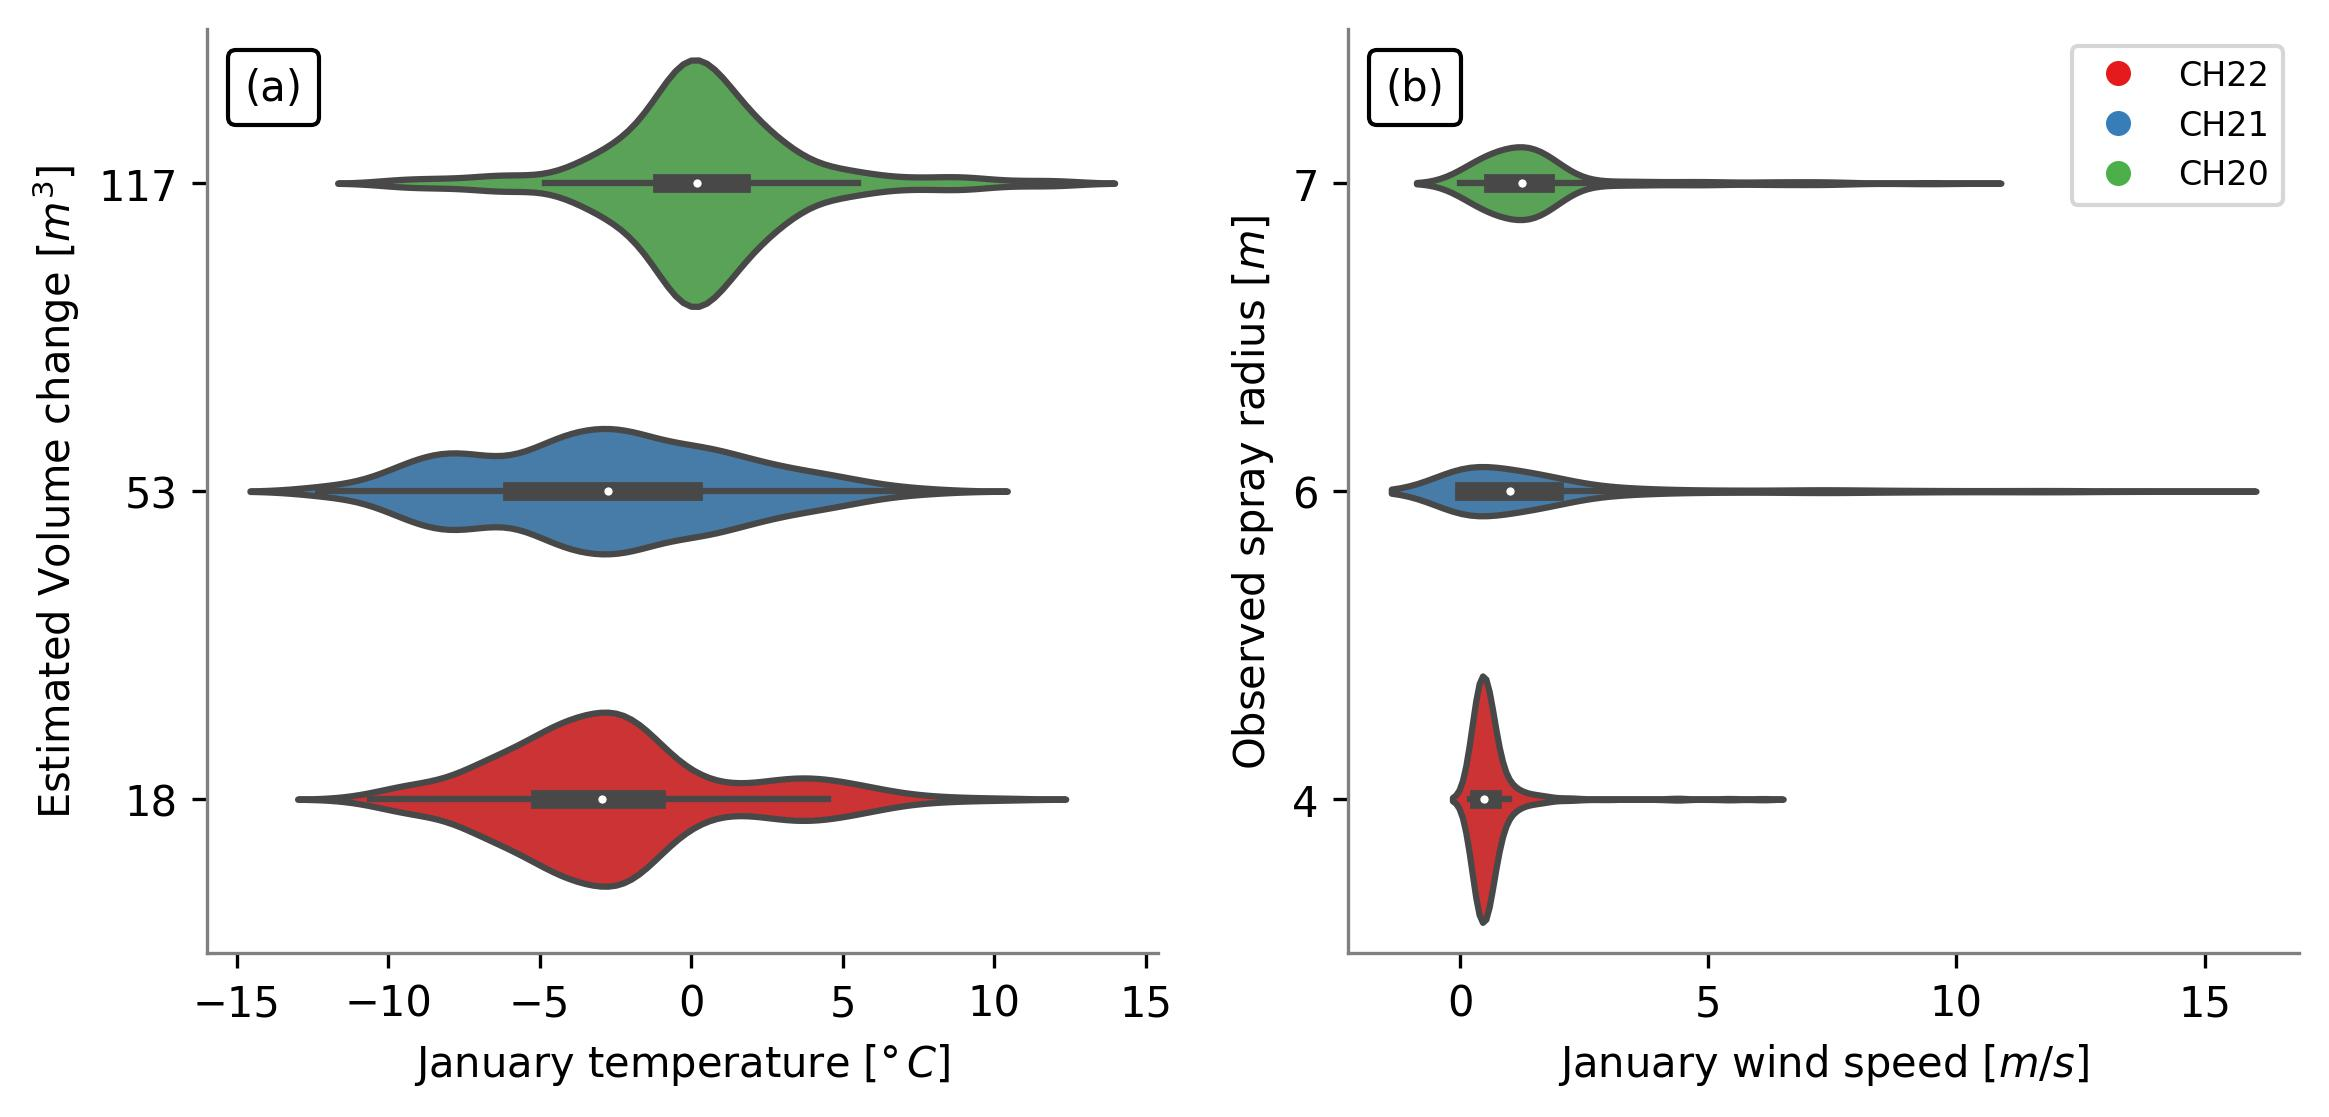
\includegraphics[width=\textwidth]{figs/CH_diffs.jpg}
\caption{(a) Estimated volume change and temperature and (b) Observed spray radius and wind speed
during January for AIRs built across three winters. } 
\label{fig:CH_diffs}
\end{figure}

AIRs built in Switzerland across three winters (CH20, CH21 and CH22) show a decreasing trend in their ice volume
changes for the month of January. Contrary to expectations, this decreasing trend was not caused by increasing
temperatures but rather by decreasing wind speeds (Fig. \ref{fig:CH_diffs}). A process-based analysis  revealed
that wind driven redistribution could explain these differences ( paper II). The influence of this process on
the fountain spray radius managed to generate AIRs six times bigger in spite of temperatures being 3 $\degree C$
warmer ( Fig. \ref{fig:CH_diffs} (b)). 



\section{Metrics to judge site suitability}

Accordingly, we propose two sets of guidelines to constrain future construction sites in a regional and a local
scale. 

\subsection{Regional scale}


The values presented are determined based on past construction experiences and can be used as guidelines to
avoid construction attempts in unfavourable sites.

\begin{enumerate}

  \item Minimum median monthly temperature less than $0 \degree C$. 
  \item Water supply with median discharge rate more than $2\, l/min$.
  \item Terrain slope between water source and site greater than 10 m every km. 

\end{enumerate}

\subsection{Local scale}

Given a valley or a region satisfying the above requirements, further selection of sites around the particular
water supply can be performed using the criterions below: 

\begin{enumerate}
  \item Water source temperature is higher.
  \item Daylight hours are lower due to shadows.
  \item Altitude is higher.
\end{enumerate}


% Such villages are expected to produce AIRs that supply daily meltwater in the order of thousands of litres for 2
% months. 

% Different forms of AIRs show different sensitivities to each of these requirements. This is discussed in the
% next chapter.

% \subsection{Water supply}

% The water source of an AIR could be either a spring or a stream. Springs are the ideal water source since they
% are easy to transport via pipelines to the construction site due to their relatively warm temperatures. Other
% water sources have higher risks of freezing events in the fountain pipeline.

% \begin{itemize}
%   \item {\bf Water supply} : The water source of an AIR could be either a spring or a stream. Springs are the ideal
%     water source since they are easy to transport via pipelines to the construction site due to their relatively
%     warm temperatures. Other water sources have higher risks of pipeline freezing events. 

%   \item {\bf Weather conditions} : AIRs prefer colder, drier and less-cloudy regions. Correspondingly,
%     temperature, humidity and number of cloud-free days during the construction period can be used to rank
%     different sites. 

%   \item {\bf Topography} : AIRs prefer shadowed valleys. This is because these landforms have lower sunshine
%     hours which is the major driver of the melting rate of all the AIRs studied in this thesis.

% \end{itemize}

% This imposes several meteorological and topographical requirements for the chosen
% construction location. The meteorological requirements can be used to identify favourable regions worldwide
% whereas the topographical requirements can be used to pinpoint the construction site within the respective
% region. Below we detail these requirements and propose methodologies for finding construction sites satisfying
% them. 
  % \item Daylight hours are lower.
  % \item Cloudy days are lower.
  % \item Temperature is lower.
  % \item Humidity is lower.

% The ice reservoir technology has found limited adoption in regions beyond Ladakh. However, this

% It remains to be  n where else AIRs can be of utility.

% AIRs cannot be built anywhere. They require weather conditions cold enough to amass a seasonal stock of ice. The
% weather suitability of locations can be identified using the model developed in paper I. But such a methodology
% has a data requirement often incompatible with what is available. Reanalysis datasets like ERA5 can serve as 

% The utility of AIRs depends on their daily meltwater discharge. 

% Temperature based 

% AIRs exhibit significant interannual, interregional and intraregional volume variations depending on the
% suitability of the location 

% In this chapter, we attempt to quantify these requirements by examining the magnitude of these differences
% across the AIRs built in India and Switzerland. We also discuss strategies to judge the utility of AIRs in new
% locations.

% The spatial and temporal variation in weather conditions determine the growth rate of AIRs. In this section, we
% instead perform a qualitative analysis of the influence of interannual, interregional and intraregional
% variations in weather conditions on the AIR growth rate based on the Indian and Swiss AIR datasets.
